% !TEX root = main.tex
\section{Core Nebulas Rank}

Core Nebulas Rank is used to measure the contributions a user to the whole economy {\textbf{in a certain period of time}}.
It is quite complicate to calculate the contribution precicesly, so we provide an approximation algorithm for it.
In this approximation algorithm, we consider two critical factors, the coinage and the position information in the transaction network. We will proof the effectiveness of the approximation algorithm in the evluation section below.

We use the transaction history on the mainnet in a certain period as the data source of Core Nebulas Rank.
All the transactions in a period of time $[t_0\ −\ T,\ t_0]$, can be specify as a set
\begin{align}
\Theta(t_0) = \{(s, t, w, \tau)\ |\ t_0 - T \le \tau \le t_0\ \land \ w > 0 \land s \neq t \}
\end{align}
\noindent Based on $\Theta(t_0)$, we can define a weighted directed graph, the node is the address of the account, the edge from node $s$ to node $d$ represents one transaction,
the weight of the edge is $w$, the time of the edge is$\tau$.

For account $a \in \mathcal{A}$, the calculation of Core Nebulas Rank$\mathcal{C}(a)$ is based on $\Theta(t_0)$, which is
\begin{align}
\mathcal{C}(a) = \Omega(\beta(a)) \times{} \Psi(\gamma(a))
\label{eq:rank}
\end{align}
\noindent $\beta(a)$ is the median stake of account $a$ in a certain period; $\gamma(a)$ is the in-and-out degree of account $a$ in a certain period.

\whitepaper{Different from the way we calculate the Core Nebulas Rank in Nebulas white paper~\cite{Nabulas}, we made some updates blow:\\
1. Don't use the top $K$ highest transaction amount as the weight when building the transaction graph; \\ 
2. Don't rely on the weight of nodes in LeaderRank to get the importance of the node. \\
First, we remove the loops before we calculate the in-and-out degree $\beta$, so it can resist from loops attack, in the same time still consider the strength of the edge. for some cases of homogeneous topology graph, PageRank and some other symatric function (such as LeaderRank) has been proof that they can't resist from sybil attack~\cite{cheng2005sybilproof}. In this yellow paper, we didn't use the Topology-like ranking stratigies. We proposed a asymatic calculation function\ref{eq:rank-param} which is effective reduce the rewards by faking the low stake nodes in \refsec{sec:function}.} 

Below, we are going to discuss three issues in ~\ref{eq:rank}: Account Median Stake $\beta(a)$, In-and-Out Degree $\gamma(a)$, and selection of function $\Omega$ and $\Psi$.

\subsection{Account Median Stake$\beta(a)$}
In time period of $[t_0\ −\ T,\ t_0]$, there are $n$ blocks in the blockchain system, marked as
\[
B_0, B_1, \dots, B_n
\]
\noindent $B_{i}$ is the parent block of $B_{i+1}$. For account $a \in \mathcal{A}$, the balance of the account at end of each block is
\[
d^a_0, d^a_1, \dots, d^a_n
\]
We can get a new list by sorting the items ascending 
\[
d^a_{(0)}, d^a_{(1)}, \dots, d^a_{(n)}
\]
$d^a_{(i)} < d^a_{(i+1)}, 0\le i \le {n-1}$, so, it easy to know,
\begin{align}
\beta(a) = \left\{ \begin{array}{rcl}
{d^a_{(k)}} & \mbox{for} & n=2\times{}k, k=1, 2, 3, \ldots \\
{(d^a_{(k)} + d^a_{(k+1)})/2} & \mbox{for} & n=2\times{}k + 1, k=1, 2, 3, \ldots
\end{array}\right.
\end{align}
The account median stake represents the coinage in a certain way, that means the account need to hold the stake more than half of the time period.

\subsection{In-and-Out Degree$\gamma(a)$}
Consider the attacker would increase the In-and-Out degree using loop attack, so, we will need to remove the forwarding loop before we calculate the In-and-Out degree for the transaction graph. Forwarding loop is a loop of transaction in a sequential of time.
The forwarding loop starts and ends on same node $v$, it is a set of edges in the transaction graph, mark it as $H(v)$, which is

\[
H(v) = \{(v, v_1, w_1, \tau_1), (v_1, v_2, w_2, \tau_2), \dots, (v_i, v_{i+1}, w_{i}, \tau_i), \dots, (v_n, v, w_{n+1}, \tau_{n+1})\}
\]
\noindent $\forall 1\le i \le n : \tau_i \le \tau_{i+1} $.
\noindent As shown in ~\ref{fig:loop}, contains a forwarding loop, please note, $(v_1, v_2, 100, 5)$ are not included in the forwarding loop.

\begin{figure}
\centering
  \begin{tikzpicture}
\pgfmathsetmacro{\XTD}{3.8}
\pgfmathsetmacro{\XMD}{1.2}
\pgfmathsetmacro{\YTD}{3.8}


\tikzset{
  node/.style={draw, circle, on grid, align=center, minimum height=2ex},
  thread/.style={draw, rectangle, on grid, align=center,color=gray!30,
  fill=gray!30,
  rounded corners,
  minimum height=3ex,fit=#1},
}

\node[node] (v) at (0, 0) {$v$};
\node[node] (v1) at (0, \YTD) {$v_1$};
\node[node] (v2) at (\XTD, \YTD) {$v_2$};
\node[node] (v3) at (\XTD, 0) {$v_3$};

\draw[->,>=stealth'] (v) to [out=135, in=225] node[left, midway] {$w=100$,$\tau=1$} (v1);
\draw[->,>=stealth'] (v1) to [out=45, in=135] node[above, midway] {$w=10$,$\tau=2$} (v2);
\draw[->,>=stealth'] (v1) to [out=315, in=225] node[below, midway] {$w=100$,$\tau=5$} (v2);
\draw[->,>=stealth'] (v2) to [out=315, in=45] node[right, midway] {$w=10$,$\tau=3$} (v3);
\draw[->,>=stealth'] (v3) to [out=225, in=315] node[below, midway] {$w=10$,$\tau=4$} (v);

\node at (2.5*\XTD, 0.5*\YTD) {
$\begin{aligned}
     H(v) = \{&(v, v1, 100, 1),\\
     &(v1, v2, 10, 2), \\
     &(v2, v3, 10, 3), \\
     &(v3, v, 10, 4) \}
  \end{aligned}$};
\end{tikzpicture}

\caption{loop\label{fig:loop}}
\end{figure}

\begin{figure}
\centering
\begin{tikzpicture}
\pgfmathsetmacro{\XTD}{3.8}
\pgfmathsetmacro{\XMD}{1.2}
\pgfmathsetmacro{\YTD}{3.8}


\tikzset{
  node/.style={draw, circle, on grid, align=center, minimum height=2ex},
  thread/.style={draw, rectangle, on grid, align=center,color=gray!30,
  fill=gray!30,
  rounded corners,
  minimum height=3ex,fit=#1},
}

\node[node] (v) at (0, 0) {$v$};
\node[node] (v1) at (0, \YTD) {$v_1$};
\node[node] (v2) at (\XTD, \YTD) {$v_2$};
\node[node] (v3) at (\XTD, 0) {$v_3$};
\draw[->,>=stealth'] (v) to [out=135, in=225] node[left, midway] {$w=90$,$\tau=1$} (v1);
\draw[->,>=stealth'] (v1) to [out=315, in=225] node[below, midway] {$w=100$,$\tau=5$} (v2);

\end{tikzpicture}
\caption{\reffig{fig:loop}去掉交易环后的交易图 \label{fig:no-loop}}
\end{figure}


After identify the forwarding loop, we need to remove the loop before use it. For example there are $n$ forwarding loop in the system, list the forwarding loop by the sequential of occurence as below:
\[
H^1(v_1), H^2(v_2), \dots, H^n(v_n)\]
\noindent The minimal amount of the transaction in $H^i(v_i)$ is $(s^i_m, t^i_m, w^i_m, \tau^i_m)$, which is,
\[
\forall (s^i, t^i, w^i, \tau^i) \in \mathcal{T} : w^i \ge w^i_m
\]
\noindent Later, for each transaction in $H^i(v_i)$, we need ot minus the minimal transcation amount $w^i_m$ accordingly,
if the latest transaction amount is 0, then remove this transaction, which is
\[
\mathcal{E}((s, t, w, \tau), w_m) = \left\{ \begin{array}{rcl}
(s, t, w-w_m, \tau) & \mbox{if} & w \ne w_m \\
\phi & \mbox{if} & w = w_m
\end{array}\right.
\]
\begin{align}
\Theta^{\prime}(t_0)=\Theta(t_0)-H^i(v) \cup \{\mathcal{E}(t), t\in H^i(v_i)\} \quad i = 1, 2,\dots, n
\end{align}
\noindent As shown in \reffig{fig:no-loop} is a transaction graph \reffig{fig:loop} after remove the forwarding loop.

%在去除所有的交易环后,对交易图中的每个节点,我们仅保留交易量最高的$k$个出边及入边,由此得到新的交易图$\Theta^{\prime\prime}(t_0)$。

Set the transfer-in amount of node $v$ is $p(v)$, then
\begin{align}
p(v) = \sum_{(s_i, v, w_i, \tau_i) \in \Theta^{\prime}(t_0)}{w_i}
\end{align}
\noindent Same reason, transfer-out amount of node $v$ is
\begin{align}
q(v) = \sum_{(v, t_i, w_i, \tau_i) \in \Theta^{\prime}(t_0)}{w_i}
\end{align}
\noindent In this case,
for node $v$, its in degree $\gamma(v)$ is

\begin{align}
\mathcal{G}(v) = (p(v) + q(v)) \cdot e^{-2\sin^2{(\frac{\pi}{4} - \arctan\frac{q(v)}{p(v)})}}
\end{align}
\noindent The curve of the function is shown as ~\reffig{fig-surf}.
\begin{figure}
  \centering
  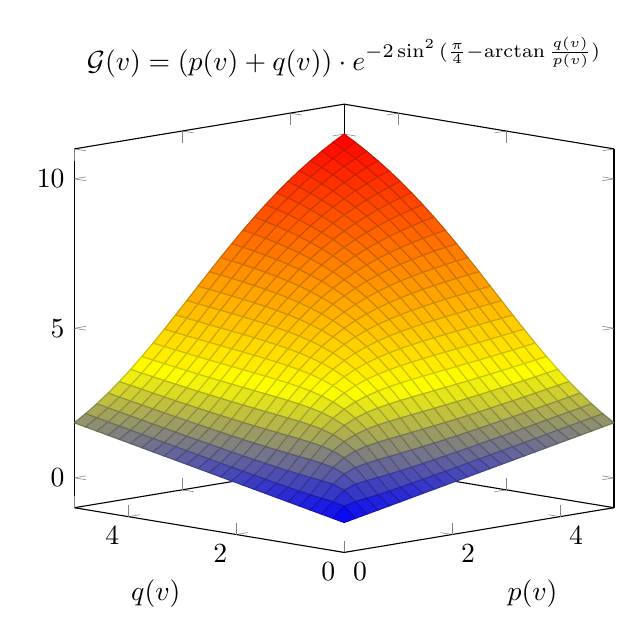
\begin{tikzpicture}[
    declare function={tf(\x)=(pi/4-rad(atan(\x)));},
    declare function={func(\x,\y)=sin(tf(\y/\x)*180/pi);}
]
\begin{axis}[
    view={315}{10},
    title={$
\mathcal{G}(v) = (p(v) + q(v)) \cdot e^{-2\sin^2{(\frac{\pi}{4} -
\arctan\frac{q(v)}{p(v)})}}$},
    xlabel=$p(v)$,
    ylabel=$q(v)$,
]

\addplot3 [
        surf,
        domain=0:5,
        domain y=0:5,
    ] {(x+y)*exp((-2)*(func(x,y))^2)};
\end{axis}
\end{tikzpicture}

\caption{The curve of the In-and-Out degree function \label{fig-surf}}
\end{figure}

\begin{align}
\gamma(v) = (\frac{\theta\cdot \mathcal{G}(v)}{\mathcal{G}(v) + \mu})^{\lambda}
\end{align}
\noindent $\theta, \mu, \lambda$ are the paramaters to be determined.


\subsection{Calculation Function \label{sec:function}}
It would extremently complicated to calculate Nebulas Ranking if we consider different usage case and its properities. However, we can provide a general function for Nebulas Rank.

We define the Nebulas Rank funciton as \(f(x)\), and \(x\) is the factor of Nebulas Rank, it can be account stake, coinage or the in-and-out degree. $f(x)$ need to satisfy flowing two properties:

\begin{property}
\label{prop:one}
For any two vailables $a$, $b$, which larger $0$, the sum of the two functions is smaller than the function of sum of two availables.
%对于任意输入$x$,将其拆分后的计算函数之和小于原计算函数。
\end{property}

\begin{align}
f(a+b)>f(a)+f(b) \quad a>0,b>0
\end{align}

\begin{property}
\label{prop:two}
For any two availables are infinity, the sum of the two functions is approxmately to the function of the sum of the two variables.
\end{property}

\begin{align}
\lim\limits_{a \to \infty, b\to \infty} f(a+b) = f(a) + f(b)\quad a>0, b>0
\end{align}

\noindent The properties described above ensure, under given transaction behaviors, the benefits of splitting stakes into smaller accounts is smaller than stay in single account, at same time, when the stake is larger enough, the cost of splitting the stakes into small accounts can be ignored. 

\noindent There are more than one functions satisfy the two properities above, In this yellow paper, we provide one of them, the curve of the function is shown \reffig{fig-nr}.
\begin{align}
f(x) = x/(1 + e^{a + b\cdot x}) \quad a>1,b<0
\end{align}
\noindent {For detailed proof, please check appendix~\ref{sec:appendix_proof}}

\begin{figure}
\centering
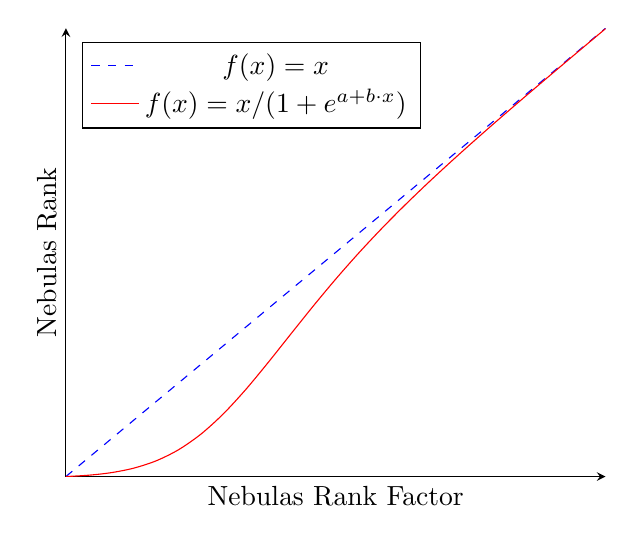
\begin{tikzpicture}[
    declare function={func(\x,\mu) = (\x / (1 + exp(\mu-\x)));},
    declare function={linefunc(\x) = \x;}
]
\begin{axis}[
    axis lines=left,
    enlargelimits=upper,
ticks=none,axis x line=bottom,axis y line=left,xlabel={Nebulas Rank Factor},
  ylabel={Nebulas Rank},
      legend pos=north west,
legend style={fill=none}
]
\addplot [dashed, domain=0:10, blue] {linefunc(x)};
\addplot [smooth, domain=0:10, red] {func(x,3)};
\addlegendentry{$f(x)=x$}
\addlegendentry{$f(x)=x/(1 + e^{a + b\cdot x})$}
\end{axis}
\end{tikzpicture}
\caption{The curve of the Nebulas Rank function \label{fig-nr}}
\end{figure}


\vspace{2em}
In summary, ~\ref{eq:rank} can be simply as below

\begin{align}
\label{eq:rank-param}
\mathcal{C}(v) =  \frac{\beta(v)}{1+e^{a + b \cdot \beta(v)}} \cdot \frac{\gamma(v)}{1+e^{c + d \cdot \gamma(v)}}
\end{align}
\noindent $a, b, c, d$ are parameters to be determined.

In order to verify the effectiveness of the function, we calculate the Nebulas Rank for all the accounts in Ethereum in certain period of time. We collected all the transaction records from May 1st 2017 to June 30th 2017 (block height: from 3629091 to 3955158), beside the transaction data, we also collected average daily price (to USD) and volumns ~\cite{coinmarketcap}.

\reffig{fig-eth-simu} shows the trending of price and Nebulas rank of the Ethereum, as shown in the picture, the black solid lines are daily volumn and average price (to USA dollar) of Ethereum, while the red solid lines represents the overall Nebulas Rank score in whole Ethereum using\ref{eq:rank-param}.

We can see, the Nebulas Rank reflects the the price changes of Ethereum very well, The correlation coefficient is 0.84427, $p$ (p-value) is $4.48\times{}10^{-17}<0.001$. That means, the function ~\ref{eq:rank}reflects the contributions of the users very well. In the other words, it demostratet the correctness of Nebulas Rank. 

\begin{figure}
\centering
\begin{tikzpicture}
  \begin{axis}[
  axis y line*=left,
  axis x line=none,
%ticks=none,
ylabel={Price of Ethereum(USA Dollars)},
%xtick={0,10,20,30,40,50,60},
%xlabel={Time(Day)}
legend style={fill=none}
    ]
\addplot[smooth, mark=., color=red] table [x=day, y=nr, col sep=comma]
    {../common/eth_simu.csv};
\label{plot_one}

\end{axis}
  \begin{axis}[
%ticks=none,
legend pos=north west,
%ylabel={Nebulas Rank},
xlabel={Time(day)},
xtick={0,10,20,30,40,50,60},
ytick={1,2},
axis y line*=right,
legend style={fill=none}
    ]
    \addlegendimage{/pgfplots/refstyle=plot_one}\addlegendentry{Nebulas Rank}

    \addplot[smooth, mark=x] table [x=day, y=cap, col sep=comma]
    {../common/eth_simu.csv};
    \label{plot_two}
      \addlegendentry{Price of Ethereum}
\end{axis}

\end{tikzpicture}
\caption{The price and Nebulas Rank of Ethereum}
\label{fig-eth-simu}
\end{figure}
